%==============================================================================
% PROJECT ASSESSMENT FORMS
%==============================================================================

\newfontfamily\assessmentarabicfont[Script=Arabic,Scale=1.0]{Times New Roman}

\newcommand{\assessmentline}[1]{\makebox[#1]{\dotfill}}

\newcommand{\assessmentHeader}{%
  \noindent
\includegraphics[width=\textwidth,height=0.48cm]{assets/forms/evaluation_header.jpeg}\par
  \vspace{0.16cm}
  \noindent\begin{minipage}[c]{0.2\textwidth}
    
\includegraphics[height=1.42cm]{assets/forms/quality_logo.png}
  \end{minipage}
  \hfill
  \begin{minipage}[c]{0.36\textwidth}
    \centering
    \rule{0.98\linewidth}{0.4pt}
  \end{minipage}
  \hfill
  \begin{minipage}[c]{0.31\textwidth}
    \raggedleft
    
\includegraphics[height=1.22cm]{assets/forms/evaluation_logos.png}
  \end{minipage}
  \par\vspace{0.16cm}
}

\newcommand{\assessmentFooter}{%
  \begin{tikzpicture}[remember picture,overlay]
    \node[anchor=south,align=center,text=gray,text width=15.7cm]
      at ([yshift=0.42in]current page.south)
      {\begin{RTL}
       {\assessmentarabicfont\fontsize{7.5}{8.5}\selectfont
       ص.ب. 11795 عين حلوان - القاهرة - مصر\\
       تليفون: 02 28162000 \hspace{1cm} تليفاکس: 02 25552468\\
       E-mail: qua-unit-sci-he@science.capu.edu.eg \hspace{0.5cm}
       Website: http://sci.capu.edu.eg/}
       \end{RTL}};
  \end{tikzpicture}%
}

\newcommand{\assessmentWatermark}{%
  \begin{tikzpicture}[remember picture,overlay]
    \node[opacity=0.06,anchor=south west] at ([xshift=-1.08cm,yshift=0.27cm]current page.south west)
      {
\includegraphics[width=7.35cm]{assets/forms/quality_logo.png}};
    \node[opacity=0.07,anchor=south east] at ([xshift=1.12cm,yshift=0.38cm]current page.south east)
      {
\includegraphics[width=7.65cm]{assets/forms/quality_logo.png}};
  \end{tikzpicture}%
}

\newcommand{\letterformgeometry}{%
  \clearpage
  \pdfpagewidth=8.5in
  \pdfpageheight=11in
  \newgeometry{left=1in,right=1in,top=0.33in,bottom=0.22in,headheight=0pt,headsep=0pt,footskip=0pt}%
}

\newcommand{\restoreaivgeometry}{%
  \clearpage
  \restoregeometry
  \pdfpagewidth=210mm
  \pdfpageheight=297mm
}

\newcommand{\projectmarkspage}{%
\clearpage
\thispagestyle{empty}
\begingroup
\small
\centering
{\Large\bfseries Project Marks\par}
\vspace{1cm}

\begin{tabular}{|C{2.2cm}|L{4.9cm}|C{2.75cm}|C{2.55cm}|C{2.85cm}|}
\hline
\textbf{ID} & \textbf{Name} & \textbf{Oral Presentation (20)} & \textbf{Participation (20)} & \textbf{Quality of Project (60)} \\
\hline
352250706 & Armia Gamal Fakry & \dotfill & \dotfill & \dotfill \\
\hline
352250808 & Sherif Karam Zaki & \dotfill & \dotfill & \dotfill \\
\hline
352250785 & Sara Essam Ibrahim & \dotfill & \dotfill & \dotfill \\
\hline
352250783 & Ziad Walid Mokhtar & \dotfill & \dotfill & \dotfill \\
\hline
352250804 & Shada AymanEldin Ahmed & \dotfill & \dotfill & \dotfill \\
\hline
352250738 & Peter Bolbol Sefin & \dotfill & \dotfill & \dotfill \\
\hline
352250787 & Salsabel Esmail Hussin & \dotfill & \dotfill & \dotfill \\
\hline
\end{tabular}

\vspace{1.35cm}
{\large\bfseries Assessment Committee\par}
\vspace{0.55cm}

\begin{tabular}{|L{7.3cm}|C{6.5cm}|}
\hline
\textbf{Name} & \textbf{Signatures} \\
\hline
Prof. Morad Rafaat & \dotfill \\
\hline
Prof. Ahmed Ezzat Labib & \dotfill \\
\hline
Prof. Rashad Abdalaaty & \dotfill \\
\hline
\end{tabular}

\vfill
\raggedright
\textbf{Date of Approval:} \rule{5.3cm}{0.4pt}
\par
\endgroup
}

\newcommand{\researchprojectevaluationform}{%
\letterformgeometry
\thispagestyle{empty}
\assessmentWatermark
\begingroup
\assessmentarabicfont
\fontsize{8.75}{10.05}\selectfont
\setlength{\parskip}{0.08em}
\setlength{\tabcolsep}{3.2pt}
\renewcommand{\arraystretch}{1.04}
\assessmentHeader
\begin{RTL}
\centering
{\fontsize{15}{17}\selectfont\bfseries استمارة تقييم مقرر المشروع البحثي للمستوي الرابع\par}
\vspace{0.16cm}

\raggedleft
\textbf{الفصل الدراسي:} الثاني \hfill \textbf{العام الاكاديمي:} 2025-2026\par
\textbf{القسم:} رياضة \hfill \textbf{البرنامج:} الإحصاء و الحاسب\par
\textbf{عنوان المشروع:} \LR{Nabta Plant Disease Analysis System}\par
\textbf{اسم الطالب:} \assessmentline{9.8cm}\par

\vspace{0.18cm}
\centering
{\bfseries لجنة المناقشة الشفوية وتقييم تقرير المشروع\par}
\vspace{0.06cm}
\begin{tabular}{|C{6.12cm}|C{4.55cm}|C{5.82cm}|}
\hline
\textbf{الاسم} & \textbf{الصفة} & \textbf{التوقيع} \\
\hline
ا.د. مراد رأفت & المشرف & \\
\hline
ا.د. أحمد عزت لبيب & عضو لجنة التقييم & \\
\hline
ا.د. رشاد عبد العاطي & عضو لجنة التقييم & \\
\hline
\end{tabular}

\vspace{0.16cm}
\raggedleft
{\bfseries درجة المقرر :}\par
\vspace{0.05cm}
\centering
\begin{tabular}{|C{8.42cm}|C{8.08cm}|}
\hline
درجة المتابعة الدورية & \\
\hline
درجة جودة التقرير البحثي (60) & \\
\hline
درجة المناقشة (20) & \\
\hline
المجوع & \\
\hline
\end{tabular}

\vspace{0.16cm}
{\bfseries نقاط تقييم المناقشة الشفوية والعرض\par}
\vspace{0.05cm}
\begin{tabular}{|C{1.73cm}|C{1.79cm}|C{4.8cm}|L{8.16cm}|}
\hline
\textbf{الدرجة الممنوحة} & \textbf{الدرجة الكلية} & \textbf{المعيار} & \centering\arraybackslash\textbf{الوصف} \\
\hline
\multicolumn{4}{|c|}{\bfseries نقاط تقييم جودة العرض التقديمي (في حالة تعدد الطلاب على المشروع توحد لكل الطلاب)} \\
\hline
 & 3 & جودة العرض التقديمي & تنظيم الشرائح، وضوح الخطوط والأشكال.\par التسلسل المنطقي للمحتوى. \\
\hline
\multicolumn{4}{|c|}{\bfseries نقاط تقييم المناقشة الشفوية والعرض (لكل طالب درجته الخاصة وإن تعدد الطلاب على المشروع الواحد)} \\
\hline
 & 4 & الإلمام بموضوع المشروع & قدرة الطالب على شرح أهداف المشروع وخلفيته العلمية ومنهجيته بوضوح. \\
\hline
 & 3 & مهارات الإلقاء والتواصل & وضوح الصوت، الثقة بالنفس، التواصل البصري.\par واستخدام لغة علمية مناسبة. \\
\hline
 & 2 & إدارة الوقت & الالتزام بالوقت المحدد للعرض دون إطالة أو اختصار مخل. \\
\hline
 & 3 & فهم النتائج وتحليلها & القدرة على تفسير النتائج ومناقشتها وربطها بأهداف المشروع. \\
\hline
 & 2 & الإجابة عن أسئلة لجنة المناقشة & دقة الإجابات وسرعة الاستجابة وإظهار الفهم للموضوع. \\
\hline
 & 1 & التفكير النقدي وحل المشكلات & القدرة على تبرير الاختيارات المنهجية. \\
\hline
 & 3 & المساهمة الشخصية في المشروع & إظهار دور الطالب الفعلي في تنفيذ العمل والنتائج المتحصل عليها. \\
\hline
 & 2 & الالتزام بالأخلاقيات العلمية & توثيق المراجع واحترام حقوق الملكية الفكرية.. \\
\hline
 & 20 & المجموع & \\
\hline
\end{tabular}
\end{RTL}
\assessmentFooter
\endgroup

\letterformgeometry
\thispagestyle{empty}
\assessmentWatermark
\begingroup
\assessmentarabicfont
\fontsize{9.2}{10.8}\selectfont
\setlength{\parskip}{0.12em}
\setlength{\tabcolsep}{3.5pt}
\renewcommand{\arraystretch}{1.32}
\assessmentHeader
\begin{RTL}
\centering
{\fontsize{13.5}{15}\selectfont\bfseries نقاط تقييم جودة التقرير البحثي\par}
{\fontsize{9.2}{10.6}\selectfont
(في حالة تعدد الطلاب على المشروع توضع نفس الدرجة لكل الطلاب المشاركين)\par}
\vspace{0.14cm}
\begin{tabular}{|C{1.73cm}|C{1.7cm}|C{4.81cm}|L{8.25cm}|}
\hline
\textbf{الدرجة الممنوحة} & \textbf{الدرجة الكلية} & \textbf{المعيار} & \centering\arraybackslash\textbf{الوصف} \\
\hline
 & 3 & الابتكار والأصالة & فكرة تطبيقية او جديدة \\
\hline
 & 5 & المحتوى العلمي والفني & وضوح أهداف المشروع. \\
\hline
 & 12 & المنهجية وتنفيذ العمل & وضوح خطوات العمل، والتجارب أو التصميمات المستخدمة، ومدى مناسبة المنهجية لتحقيق أهداف المشروع. \\
\hline
 & 12 & النتائج والمناقشة & جودة عرض النتائج، وتحليلها وتفسيرها، وربطها بأهداف المشروع والدراسات السابقة. \\
\hline
 & 12 & تنظيم التقرير وجودة الكتابة & ترتيب الفصول، وسلامة اللغة، وجودة الجداول والأشكال، والالتزام بقواعد التنسيق الأكاديمي. \\
\hline
 & 10 & التوثيق و الاستنتاجات & توصيات أو مقترحات مستقبلية مناسبة. \\
\hline
 & 6 & الالتزام باخلاقيات المهنة & توثيق المراجع واحترام حقوق الملكية الفكرية وعدم المبالغة في النتائج \\
\hline
 & 60 & المجموع & \\
\hline
\end{tabular}

\vspace{0.32cm}
\raggedleft
{\bfseries الدرجة الممنوحة هي متوسط درجات أعضاء اللجنة لكل بند}
\end{RTL}
\assessmentFooter
\endgroup
}

\newcommand{\researchprojectevaluationpdf}{%
  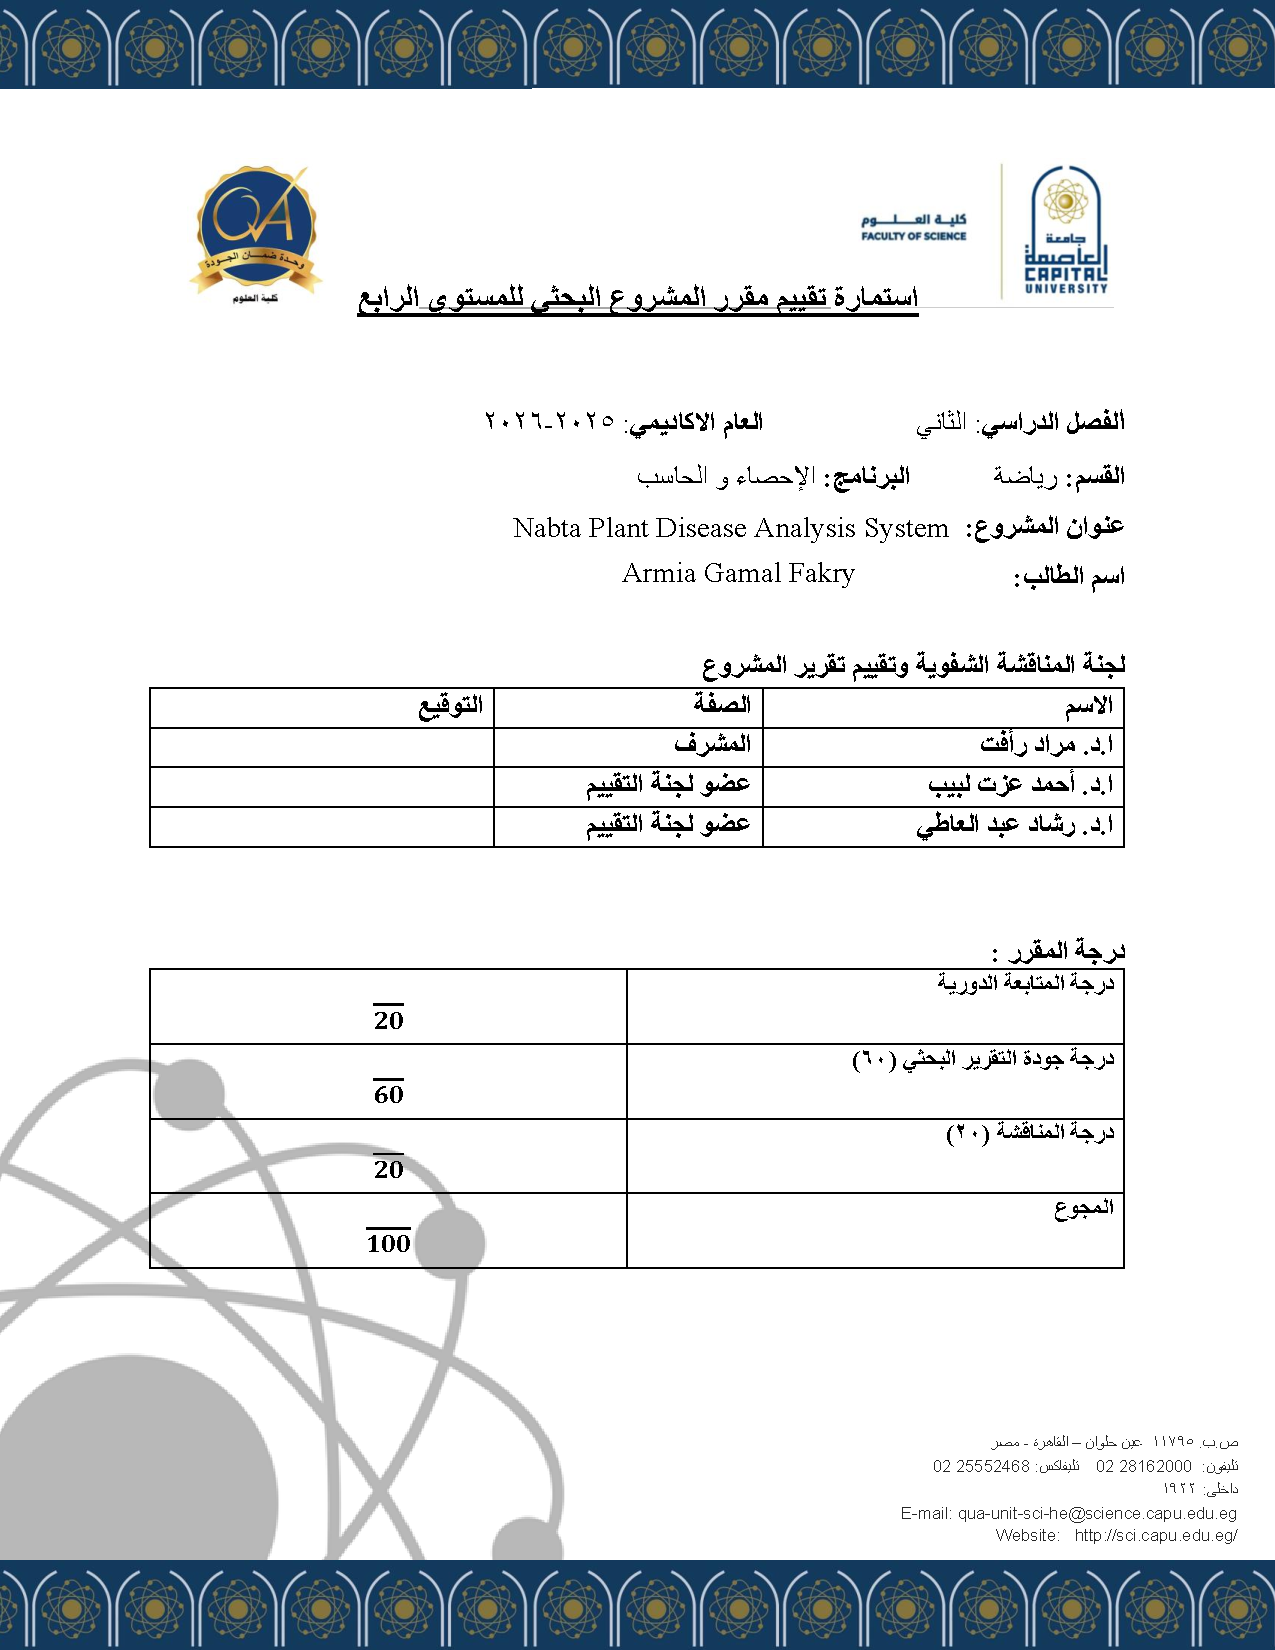
\includepdf[
    pages=-,
    fitpaper=true,
    pagecommand={\thispagestyle{empty}}
  ]{assets/forms/research_project_evaluation_forms_filled.pdf}%
}

\projectmarkspage
\researchprojectevaluationpdf
\restoreaivgeometry
